% Document
% Document
\documentclass[12pt, a4paper]{article}
\usepackage[T1]{fontenc}
\usepackage[utf8]{inputenc}
\usepackage{authblk}
\usepackage{lipsum}
\usepackage{tikz}

% Figure and table formating
\usepackage{epsfig}
\usepackage{tabu}
\usepackage{rotating}
\usepackage{pbox}
\usepackage{framed, multicol}
\usepackage[framemethod=TikZ]{mdframed}

% Set up Frame
\mdfdefinestyle{MyFrame}{%
    linecolor=black,
    skipabove=10pt,
    outerlinewidth=2pt,
    roundcorner=20pt,
    innertopmargin=10pt,
    innerbottommargin=10pt,%\baselineskip,
    innerrightmargin=20pt,
    innerleftmargin=20pt,
    backgroundcolor=gray!50!white}

\usepackage{float}
\usepackage[left=1 in, right=1 in, top=1.25 in, bottom=1.25 in]{geometry}

% Fonts - Mathtime
%\usepackage{txfonts}
\usepackage{amsmath} % Add amssymb if not using Mathtime

% Text
\setlength{\parindent}{0.5in}
\frenchspacing  \tolerance = 800  \hyphenpenalty = 800

\usepackage{lineno} % Line numbers
\def\linenumberfont{\normalfont\footnotesize\ttfamily}
\setlength\linenumbersep{0.1 in}

\usepackage{setspace}

% Format section and subsection headers
\makeatletter
\renewcommand{\section}{\@startsection
{section}%                   % the name
{1}%                         % the level
{0mm}%                       % the indent
{-\baselineskip}%            % the before skip
{0.5\baselineskip}%          % the after skip
{\normalfont\bf\large}} % the style

\renewcommand{\subsection}{\@startsection
{subsection}%                   % the name
{2}%                         % the level
{0mm}%                       % the indent
{-\baselineskip}%            % the before skip
{0.5\baselineskip}%          % the after skip
{\normalfont\bf}} % the style
\makeatother

% Other
\usepackage{graphicx}
\usepackage[singlelinecheck=false,font=small,labelfont=bf]{caption}

% Bibliography
\usepackage[numbers, compress]{natbib} % Bibliography - APA
\bibpunct{(}{)}{;}{a}{}{,}

% Format the Bibliography appropriately
% increase \bibhang to take care of the numbers
\setlength{\bibhang}{0pc}
\makeatletter
% patch \@lbibitem to print the current number before the authors
\patchcmd{\@lbibitem}
  {]}
  {] \theNAT@ctr. \newline }
  {}{}
\makeatother


%%%%%% FRONT MATTER %%%%%%%%%

\title{Detecting and quantifying parasite-induced host mortality from intensity data: method comparisons and limitations}
\author{Mark Wilber, Sara Weinstein, and Cherie Briggs}


\begin{document}


\maketitle

\section*{Abstract}

Parasites can often have significant impacts on host populations through parasite-induced host mortality.  Detecting and quantifying the magnitude of parasite-
induced mortality, particularly for macroparasites in which pathology is
linked to to the intensity of infection, can provide important insight into
parasite dynamics and host population management. This is, however,
notoriously difficult in practice as the only data often available are measures of parasite intensities. In this study we provide a novel method for detecting and
quantifying parasite-induced mortality in wildlife populations from intensity
data and, using simulations, we show that our method is more reliable for
detecting and quantifying parasite-induced host mortality than the methods that are
currently available.  We also show that this method provides quantitative
estimates of parasite-induced mortality in empirical data that are consist
with previously published qualitative estimates. However, we stress that this
method, along with all methods for estimating parasite-induced mortality in
host populations for intensity data alone, has a number critical assumptions that limit their
applicability in the real world.  We conclude that methods for estimating and
detecting parasite-induced mortality from intensity data should be used only as an
exploratory tool for informing more rigorous studies of parasite-induced host
mortality.

\doublespacing

\linenumbers
\section*{Introduction}

Infectious agents can have major impacts on animal populations through changing
population dynamics and stability \citep{Dobson1992}, altering predator-prey interactions \citep{Joly2004}, and
even causing species' decline and extinction \citep{DeCastro2005a,McCallum2012b}. Accurately estimating the impact
of these infectious agents in wildlife is critical to understanding what
regulates host and parasite populations, making predictions about disease
transmission, and managing disease outbreaks \citep{Langwig2015}. The impact of microparasite pathogens, such as rabies \citep{Coyne1989}, bovine TB \citep{Cox2005}, and
rinderpest \citep{Tille1991}, is typically quantified based on the presence or absence of
disease, and does not account for the number of infectious agents present.
This method is sufficient for many bacterial and viral agents that reproduce within a
host, however for macroparasites, pathology is linked to the intensity of infection and hosts cannot be simply categorized as infected and
uninfected \citep{AndersonandMay1979,Lafferty2002}.  Helminths exhibiting this intensity dependent pathology have
significant impacts on human health \citep{Brooker2004}, domestic livestock economics \citep{Roeber2013}, and
wildlife survival \citep{Kirk2003, Logiudice2003}.  While it is generally assumed that some fraction of
wild host populations must succumb to parasitic infections, it is notoriously
difficult to actually quantify parasite-induced host mortality (PIHM) in wild
animal populations \citep{McCallum2000a}.

Ideally, parasite-induced host mortality is
quantified by experimentally infecting and tracking individual hosts in the
wild population; however, for logistical and ethical reasons this method is
rarely feasible \citep{McCallum2000a}. Data on parasite intensity is much easier to collect and has
often been used to identify the presence of PIHM \citep{Crofton1971a,Lester1977,Lester1984,Lanciani1989,Royce1990,Ferguson2011} and to quantify the
relationship between infection intensity and host mortality \citep{Adjei1986}.

\cite{Crofton1971a} first proposed that PIHM could be identified by comparing the
observed parasite distribution in the host population to the distribution
predicted in the absence of parasite-induced mortality. We briefly introduce the Crofton Method here and provide a more detailed explanation of its implementation in \emph{Supplementary Material (SI)} 1. This method
assumes that, prior to host mortality, infection intensity in the host population follows a negative binomial distribution and the tail of the distribution is truncated as intensity dependent pathology removes the most heavily infected hosts. Assuming mortality occurs only in heavily infected hosts, evidence of this parasite-induced mortality should then be detectable by iteratively
fitting a negative binomial distribution to hosts with lower and lower parasite
loads, and comparing these truncated predicted distributions to the corresponding truncated observed parasite data. [FIGURE]

The Crofton Method may be able to detect the presence of PIHM, but it does not quantify the relationship between infection intensity and host survival
probability. \cite{Adjei1986} suggested that this relationship
could be calculated by first using the Crofton Method to estimate the pre-mortality parasite distribution and then using this distribution to calculate the
probability of host survival with increasing parasite intensity. To do this,
\cite{Adjei1986} modeled host survival as a logistic function and then used a generalized linear model (GLM) to estimate the logistic parameters (see \emph{SI} 2 for a technical description of the Adjei Method).
\citeauthor{Adjei1986} suggested that this method could provide an estimate for the parasite intensity at which a host has a 50\% chance of suffering parasite-induced mortalith ($LD_{50}$). However, to implement this method the observed data must be
modified to fit the GLM framework and subjectively binned when mean
infection intensity is high or sample sizes are small (see SI 2 for details).

After 30 years, and despite clear limitations \citep{McCallum2000a}, these
methods (particularly the Crofton Method) are still discussed among
parasitologists and are the primary techniques for examining population level
impacts of parasitism using parasite intensity data. In these methods, PIHM can
only be identified by visually examining plots and, with no clear decision
rule, it can be difficult to determine the significance of PIHM across
different host-parasite systems. The survival function given by the Adjei
Method offers one solution; however, this method requires manipulating the
original data and its accuracy has never been validated.

Intensity data should
be used to estimate parasite impacts on host populations only if unbiased and accurate methods exist. In
this study, we first propose a novel method for detecting and quantifying PIHM. We
next use simulations to compare our method with the previous Adjei
Method to test the ability of both to (1) detect occurrence of PIHM and (2) estimate the
lethal parasite load ($LD_{50}$) and the associated survival function.  We then
apply both methods to real datasets previously used in PIHM analyses and
compare the results. Finally, we discuss the limitations of inferring PIHM
from intensity data and whether any method for inferring PIHM has a place
in quantitative parasitology.

\section*{Methods}

\subsection*{A novel, likelihood-based method for estimating PIHM}

Here we propose a novel, likelihood-based method (henceforth Likelihood Method)
that does not require binning or data alteration, reduces the number of
parameters to be estimated, is highly generalizable, and uses standard
statistical techniques to determine PIHM significance.  The Likelihood Method
begins with the same assumptions as the Adjei Method: namely that infection of
a host, parasite-induced mortality of a host, an the sampling of a host
population occur at distinct time intervals during a hosts life. As discussed by
\citeauthor{Adjei1986}, this is not necessarily unrealistic as studies have
shown that infection and host mortality are often age and/or body size dependent [citations].

The Likelihood Method then assumes that prior to mortality the parasite distribution can be described by the distribution $g(x; \boldsymbol{\phi})$, which specifies the probability of a host having $x$ parasites when it is observed.  $\boldsymbol{\phi}$ is a vector of parameters that describes the shape this distribution.

The method then assumes that the probability of a host surviving with $x$ parasites from infection until sampling is given by $h(\text{survival} ; x, \boldsymbol{\theta})$ where $\boldsymbol{\theta}$ specifies any additional parameters needed to define the host survival function.

With these two assumptions, we can define a probability distribution that gives the probability of having a parasite load of $x$ parasites conditional on host survival.  Using standard rules of conditional probability this distribution can be written as

\begin{equation}
    P(x | \text{survival}) = \dfrac{P(\text{survival} | x) * P(x)}{P(\text{survival})}
    \label{eq:concept}
\end{equation}

$P(\text{survival} | x)$ is the survival function $h(\text{survival}; x, \boldsymbol{\theta})$, $P(x)$ is the pre-mortality parasite distribution $g(x; \boldsymbol{\phi})$ and $P(\text{survival}) = \sum_{x=0}^{\infty} P(\text{survival} | x) * P(x) =  \sum_{x=0}^{\infty} h(\text{survival}; x, \boldsymbol{\theta})  * g(x; \phi)$. Therefore equation \ref{eq:concept} can be written as

\begin{equation}
    P(x | \text{survival}) = \dfrac{h(\text{survival}; x, \boldsymbol{\theta})  * g(x; \boldsymbol{\phi})}{\sum_{x=0}^{\infty} h(\text{survival}; x, \boldsymbol{\theta})  * g(x; \boldsymbol{\phi})}
    \label{eq:dist}
\end{equation}

% \begin{equation}
%     h(x ; a, b) = \dfrac{e^{a - b \log(x)}}{1 + e^{a - b \log(x)}}
%     \label{eq:logistic}
% \end{equation}

Using this probability distribution, one can then find the parameters $\boldsymbol{\theta}$
and $\boldsymbol{\phi}$ that maximize the likelihood of an observed host-parasite dataset.
To estimate the significance of PIHM in a host-parasite system, a likelihood
ratio test can be used in which the full model is given by equation
\ref{eq:dist} and the reduced model is given by the pre-mortality distribution
$g(x; \boldsymbol{\phi})$.  If PIHM is not significant in the system, the resulting
likelihood ratio statistic should approximately follow a $\chi^2$ distribution
with degree of freedom equal to the number of parameters in the full model with parasite-induced mortality minus the number of parameters in the reduced model without parasite-induced mortality [citation].

Equation \ref{eq:dist} could be parameterized in many different ways depending
on the parasite system of interest. In this study, we adopt the typical assumption that the pre-
mortality parasite distribution $g(x; \boldsymbol{\phi})$ follows a negative binomial
distribution with the parameters mean parasite intensity ($\mu_p$) and
aggregation ($k_p$) before mortality, respectively (smaller $k_p$ indicates
more aggregation) \citep{Crofton1971a,AndersonandMay1978,Adjei1986}.   The negative binomial distribution can arise as the equilibrium parasite
distribution under a variety of different biological and statistical assumptions
\citep{Kendall1948a, Boswell1970, Calabrese2011}. However, it is also an incredibly flexible
distribution that fits many host-parasite systems regardless of whether the
underlying mechanisms lead to an exact negative binomial distribution
\citep{Shaw1998}.

Choosing an appropriate function for $h(\text{survival}; x, \boldsymbol{\theta})$ will depend on the system under consideration.  Many theoretical models of
parasite-induced host mortality assume that the parasite-induced death rate of
hosts is a linear function of parasite intensity
\citep{AndersonandMay1978,Dobson1992,Barbour2000}. It has been previously noted that parasite-induced mortality can be nearly impossible to detect from intensity data when the host survival function is a linear function of parasite intensity as the post-mortality distribution will be of a similar form as the pre-mortality distribution \citep{Lanciani1989}. For example, \cite{Barbour2000} showed that both simple host parasite models without parasite-induced host mortality and those with linear parasite-induced host mortality produced Poisson distributions at equilibrium. More complex, non-linear survival functions were needed to produce over-dispersed of under-dispersed post-mortality distributions.  This is not unrealistic as empirical evidence has shown that non-linear host-survival functions are not uncommon
\citep{Benesh2011} [phrasing].

As one of the goals of this study is to compare this new
Likelihood Method to the previously proposed Adjei Method, we adopt the host-
survival function used in their study and assume host-survival is non-linear and follows a logistic function given by

\begin{equation}
    h(\text{survival}; x, a, b) = \dfrac{e^{a - b \log(x)}}{1 + e^{a - b \log(x)}}
    \label{eq:logistic}
\end{equation}
where $b / 4$ determines the maximum rate of decline of
host survival probability with increasing parasite load, analogous to the pathogenicity parameter $\alpha$ in traditional macroparasite models \citep{AndersonandMay1978}.  When $b$ is held constant, for every one unit increase in $a$ the parasite intensity at which 99\% of hosts survive increases by $ 1/ b$.  The equation $\exp(a
/ b)$ can also be used to calculate the parasite $LD_{50}$, here defined as the
infection intensity at a host has a 50\% dying.  This function is commonly used in toxicology and survival analysis and has the useful properties of being bounded between 0 and 1 and being differentiable for all $x$.  That being said, it is phenomenological and there is little justification to use it rather than it tends to survival data. However, given that a goal of these analyses is to
compare this method's results the those given by the Adjei Method it is natural
to adopt the same host-survival function to facilitate comparison.  When
applying the likelihood method to other systems, other more mechanistic host-survival functions can be used in place of equation \ref{eq:logistic}.

\subsection*{Evaluating the Adjei and Likelihood Methods}

\emph{Question 1: Can we detect PIHM?}

We tested the ability of the Adjei and the Likelihood Methods to identify the presence of PIHM on simulated data with known pre-mortality parameters. Consistent with the assumptions of the model that parasite infection, mortality, and sampling occur at distinct life stages of the host, we first created a pre-mortality host population by drawing $N_p$ randomly infected hosts from a
negative binomial distribution with parameters $\mu_p$ and $k_p$. This is equivalent to the period of hosts becoming infected with parasites given in \cite{Adjei1986}.  In the Adjei Method and Crofton Method, $N_p$ is a necessary parameter that is defined as the number of hosts in the population before parasite-induced mortality.  A more appropriate way to define this parameter is the number of hosts that would have been sampled had parasite-induced host mortality not occurred.  This parameter is not necessary using the Likelihood Method because unlike the Adjei Method and Crofton Method which estimate parasite-induced mortality using absolute numbers of hosts, the Likelihood Method estimates parasite-induced mortality using probabilities. However, to compare the results of the Likelihood Method with the Adjei Method, we specified a value for $N_p$ for all simulations.

Second, we chose values of $a$ and $b$ for the host survival function and calculated the probability of survival
for all $N_p$ hosts using equation \ref{eq:logistic}.  Then, for each host, we drew a random number from a uniform distribution
between 0 and 1 and if the calculated host survival probability was less than this random
number, the host experienced parasite-induced mortality.  This was the period in which hosts died due to infection. The parasite distribution in these simulated surviving hosts represented the parasite distribution in a wild host population that has undergone parasite-induced host mortality.

We used these simulated pre-mortality and post-mortality datasets to test the
ability of both methods to correctly determine whether or not PIHM was
occurring when the parameters $N_p$, $\mu_p$ and $k_p$ were known.  Although
the parameters $N_p$, $\mu_p$, and $k_p$ are always unknown in real systems, a
method that fails under these ideal simulation conditions will certainly also
fail using less ideal, empirical data. In practice, for the Adjei Method, $N_p$, $\mu_p$,
and $k_p$ are estimated using the Crofton Method \citep{Adjei1986}, while $\mu_p$ and $k_p$ in
the Likelihood Method can be estimated jointly with $a$ and $b$ or via the
Crofton Method.

We used three different values of $\mu_p$ (10, 50, 100) and for each $\mu_p$ we examined three different survival functions that had gradual, moderate, and steep decreases in the host survival with increasing parasite intensity (Figure \ref{fig:question1}A).  For a given $\mu_p$, each survival function had the same $LD_{50}$ ([$\mu_p = 10$, $LD_{50} = 7.39$], [$\mu_p = 50$, $LD_{50} = 35.57$], [$\mu_p = 100$, $LD_{50}= 77.3$]),  but different values of $a$ and $b$.  We examined each $\mu_p$-survival function pair at  three levels of parasite
aggregation, $k_p = 0.1$, 0.5, and 1 --- realistic values of parasite aggregation in natural populations \citep{Shaw1998}.  For each of these parameter
combinations we simulated 150 datasets and tested the probability of each method correctly identifying PIHM in the post-mortality dataset (power) and incorrectly identifying PIHM in the pre-mortality dataset (Type I error).  For each method, we used a likelihood ratio test to determine whether the full model with PIHM provided a significantly better fit than the reduced model without PIHM at significance level of 0.05.  We tested each parameter combinations for pre-mortality population sizes of $N_p$ = [50, 100, 200, 300, 400, 500]. $N_p$ is not technically the sample size on which the methods are being
tested for the post-mortality data because PIHM reduces $N_p$ for each simulated
dataset.  We therefore used the average number of surviving hosts over all 150 simulations for a given parameter combination as our measure of sample size in the power simulations.\\

In the next simulation, we tested the ability of only the Likelihood Method to
correctly identify PIHM and estimate $LD_{50}$ when the pre-mortality
parameters are unknown.  As a best-case scenario, we simulated host-
parasite systems with $\mu_p = 10$ and $k = 1, 0.5, \text{and} 0.1$ [re-run for 0.5 and 0.1] as it is easier to detect PIHM from small samples sizes when mean parasite intensity is low. We then used
the Likelihood Method to identify PIHM for gradual, moderate and steep survival
functions when the pre-mortality parameters $\mu_p$ and $k_p$ also needed to be estimated.  We
perform 500 simulations over a range of different samples sizes following the
simulation procedure described above.

\noindent
\emph{Question 2: Can we estimate properties of the host survival function?}

In the previous section we compared the ability of the Adjei Method and the Likelihood Method to correctly identify whether or not PIHM was a occurring in a system (i.e. a yes or no answer). In this section we compare the ability of the Adjei Method and the Likelihood Method to estimate properties of the survival function such as the parameters $a$, $b$ and $LD_{50}$.  To do this, we used the same simulation procedure and parameter combinations described above. For each parameter
combination we simulated 150 datasets, estimated $a$, $b$, and $LD_{50}$ and calculated the standardized bias and
precision \citep{Walther2005} for these estimates.  Because estimating properties of the host survival function requires more information than simply detecting PIHM, we used larger values of $N_p$ for this simulation ($N_p$ = [300, 500, 1000, 2000, 5000, 7500,
10000]).  We used the average number of surviving hosts over all 150 simulations for a given parameter combination as our measure of sample size.  Because parameters $a$ and $b$ showed similar patterns of bias and precision, we only show the results for $a$.


\subsection*{Application to real data}

We tested the ability of the Adjei Method and the Likelihood Method to identify
PIHM in 6 host-parasite datasets given in \cite{Crofton1971a} and 4 datasets
given in \cite{Adjei1986} (Table \ref{table:pihm}). \citeauthor{Crofton1971a} analyzed infection patterns in the snail \emph{Gammarus pulex} infected with the
acanthocephalan \emph{Polmorphus minutus}. \citeauthor{Adjei1986} analyzed males and females of two species of lizard fish \emph{Saurida tumbil} and
\emph{S. undosquamis} that were infected by the cestode
\emph{Callitetrarhynchus gracilis}.

In both earlier studies, the authors reported PIHM in some of the datasets and we tested whether the Adjei
Method and/or the Likelihood Method also predicted PIHM. For the 6 datasets from
\cite{Crofton1971a}, we truncated the data at 4 parasites, applied the Crofton
Method to estimate the pre-mortality distribution, and then ran the Likelihood
Method and Adjei Method using these pre-mortality parameters.  For the
\cite{Adjei1986} datasets, we followed the same procedure as the authors and
first truncated the data at 2 parasites and then fit the Crofton Method for the
female fish of both species.  Then, following the original authors' methods, we parameterized the male pre-mortality
distributions for each species with the results from the females.  Finally, we
applied the Adjei Method and the Likelihood Method to determine whether or not
PIHM was significant for these species and compared our results to those given by the authors.  All fitting to data was done with the code provided in \emph{SI} 4.

\section*{Results}

\subsection*{Question 1: Detecting presence of PIHM}

The power of the Adjei Method to detect PIHM in a
system was close to unity for larger sample sizes and tended to
decrease as sample size decreased (Figure \ref{fig:question1}C; \emph{SI} 3 Figs 1-3).  The Likelihood Method had a power close to
unity for all parameter combinations and sample sizes considered.  With gradual
survival functions, the power of the Likelihood Method decreased slightly for small samples sizes (Fig. \ref{fig:question1}C, \emph{SI} 3 Figs 1-3).

The Adjei Method showed highly inflated Type I error rates (i.e. falsely detected
PIHM) for all parameter combinations that we
considered (Fig. \ref{fig:question1}B; \emph{SI} 3 Figs 1-3).  This method also showed the unintuitive pattern of Type I error
rate decreasing as sample size decreased.  This pattern was due to the issue of
binning discussed in the \emph{Introduction} and \emph{SI} 2. For small samples sizes, the
applicability of the Adjei Method is compromised without binning the observed
data in some way.  In contrast, the Likelihood Method showed a Type I
error rate at or near the pre-set level of 0.05 for all parameter combinations
and sample sizes considered (Fig. \ref{fig:question1}B; \emph{SI} 3 Figs 1-3).

\subsection*{Question 2: Estimating the $LD_{50}$ and survival function}

The Likelihood Method gave asymptotically unbiased estimates of the $LD_{50}$
for all combinations of parameters examined in this study (Fig. \ref{fig:question2}, \emph{SI} 3 Figs 4-6).  Even for
the smallest sample sizes we considered, the Likelihood Method's estimate of $LD_{50}$
was largely unbiased, with small biases occurring for host survival functions
that were gradual. The precision of the Likelihood Method's $LD_{50}$ estimates decreased
(increasing coefficient of variation) as sample size decreased for all
parameter combinations we examined (Fig \ref{fig:question2}, \emph{SI} 3 Figs 4-6).

The Adjei Method produced biased estimates of the $LD_{50}$ across nearly all parameter combinations (Fig \ref{fig:question2}, \emph{SI} 3 Figs 4-6).  For $\mu_p = 10$, the $LD_{50}$
estimates from the Adjei Method were largely unbiased for large samples sizes, but as $\mu_p$ increased, the Adjei Method
produced biased estimates of $LD_{50}$ across all sample sizes, with bias
increasing as sample size decreased (Figure \ref{fig:question2}, \emph{SI} 3 Fig 4-6). The $LD_{50}$ estimates from the Adjei
Method showed large decreases in precision with the steepest survival function across all values of $\mu_p$ (Figure \ref{fig:question2}, \emph{SI} 3 Fig 4-6).

In terms of the host survival function, the Likelihood Method gave unbiased estimates of survival function parameters when sample sizes were large, however as sample size decreased these estimates became severely biased (Fig. \ref{fig:question2}, \emph{SI} Fig 7 - 9) The Adjei Method produced
biased estimates of the host survival function across all sample sizes, with the bias
consistently being larger when the survival function was steeper and $\mu_p$ was larger (Fig \ref{fig:question2}, \emph{SI} 3 Figs 7-9).

\subsection*{Detecting PIHM with unknown pre-mortality parameters}

When all parameters were jointly estimated, the Likelihood Method showed highly
context-dependent results when detecting PIHM in the best-case scenario of
$\mu_p = 10$ and $k_p = 1$. The Likelihood Method's power of detecting PIHM was
greater than 0.8 when host sample sizes exceeded 424 and 83  for survival
functions that were moderate and steep, respectively (Fig
\ref{fig:real_power}).  When the host survival function was gradual, the
Likelihood Method never had a power greater than 0.8 for any post-mortality
samples sizes we considered (Fig \ref{fig:real_power}).

\subsection*{Application to real data}

The previous authors qualitatively detected PIHM
in 7 of the 10 datasets considered(Table \ref{table:pihm}).  The Likelihood Method parameterized
from the pre-mortality parameters of the Crofton Method detected significant
PIHM in 6 of these 7 datasets at a significance level of 0.05.  The only
dataset in which the Likelihood Method did not detect a significant effect of PIHM was the Adjei dataset
for female \emph{S. tumbil}.  For this dataset there was a marginally significant effect
of PIHM ($\chi^2_{df=2} = 5.34; p = 0.069$). The Adjei Method detected PIHM in 9 of the 10 datasets (Table \ref{table:pihm}), consistent with our simulation results that the Adjei Method has a high Type I error rate.

\section*{Discussion}


Quantifying the impact of parasitism on wild host populations is critical for managing wildlife populations and understanding parasite-host dynamics. Ideally the relationship between
infection intensity and host survival would be measured experimentally, but for
logistical and ethical reasons, this is often impossible \citep{McCallum2000a}.
Looking for evidence of mortality in parasite distribution data requires the
least amount of information, but is notoriously difficult to implement. The
methodological flaws in the Adjei Method limit its utility, so here we propose
an alternative, likelihood-based, method to estimate host survival and the
$LD_{50}$ from observed parasite intensity data.  This
method is a significant improvement over the previous methods because it requires fewer parameters,
provides a statistical decision rule for identifying PIHM and does not require
any data manipulation.

Using simulated data, we found that the Likelihood Method always out performed the Adjei Method. For simply detecting the presence of PIHM, the Likelihood
Method was both more powerful and had fewer false detection events (Type I
errors).  When both methods were applied to published datasets previously used
in PIHM analyses, the Adjei Method tended to detect PIHM where it had not previously been
reported, consistent with the high Type I error rate observed in our
simulations. The Likelihood Method was also more precise and less
biased in calculations of both the parasite $LD_{50}$ and host survival curve over the parameter values we considered.
However, while only the Likelihood Method produced precise and unbiased $LD_{50}$
estimates, neither method could provide unbiased estimates of the host survival
function at realistic sample sizes.  These simulations demonstrate that
the Likelihood Method is more powerful and precise than the previously proposed Adjei Method.

Although superior to the Adjei Method, the Likelihood Method is not universally applicable to real data.  Our simulations showed when the when pre-
mortality parameters were estimated directly, the Likelihood Method needed at
least 83-424 samples to have 80\% power for steep to moderate survival functions, an even larger sample size as the survival function became more gradual. While some of these sample sizes are reasonable for hosts such as invertebrates or small fish, even the smallest sample sizes are completely
unfeasible for many vertebrates, particularly the species of conservation
concern where addressing the impact of parasitism would be most important. An
even larger sample size would be required to identify PIHM when parasites are highly aggregated, mean infection intensity is
high, or parasite prevalence is low, all of which are
common in many parasitic helminths.  Moreover, our results are in agreement with previous work that has shown that as host-survival functions become progressively more linear, PIHM becomes all but impossible to detect \citep{Lanciani1989}.  This result, however, does not preclude the use of this method as non-linear survival functions
are not uncommon in empirical host-parasite systems \citep{Benesh2011}.  Finally,
while linear functions make PIHM undetectable, at the other extreme, steep,
non-linear survival curves produce severely biased estimates of the survival
function. Give the interaction between all of these different factors, the
Likelihood Method is probably limited to detecting PIHM in systems where greater than 100 hosts can be collected, parasites are
common and only moderately aggregated, and substantial host mortality occurs at relatively low parasite intensity.

While we have improved on the existing methods for quantifying
PIHM from parasite intensity data, all such methods require several
fundamental, and potentially problematic assumptions.  Nearly all current methods derive from \cite{Crofton1971a} \citep[but see][]{Ferguson2011} and assume that, prior to any PIHM, parasites are distributed in the host population following a
negative binomial distribution. But, it is fundamentally impossible to know
what the pre-mortality parasite distribution was in a wild host population and
it is widely recognized that different processes can lead to a variety of
parasite distributions in hosts \citep{Anderson1982a, Duerr2003}. However, the negative binomial is extremely
flexible and there is substantial empirical and theoretical evidence to support
the assumption that, prior to any PIHM, parasite distributions can be fit by a negative binomial distribution \citep{Shaw1995,Shaw1998,Wilson2002}.

Unfortunately, this
flexibility in the distribution may also reduce our ability to detect PIHM. If
a negative binomial can be fit to the observed post-mortality parasite
distribution then, regardless of how lethal the parasite was, it will be
impossible to detect PIHM because there is no need for a more complex model.
Most observed parasite distributions are well fit by the negative binomial distribution \citep{Shaw1998}, suggesting
that systems where these methods are applicable may be more the exception than
the rule.  Furthermore, even when truncation of the negative binomial distribution is detected, it may be caused by other
processes such as within host density dependence, age dependent variation in host
resistance and/or heterogeneous infection rates \citep{McCallum2000a,Anderson1982a,Rousset1996}.  This means that in the event
that PIHM is detected, it may actually not be the result of PIHM.

Given these numerous caveats, is there a place in parasitology for methods that
estimate PIHM from intensity data?  We are in agreement with
\cite{Lester1984} that, at the very least, methods for estimating PIHM can
provide preliminary insight into whether or not PIHM is worth further
exploration.  However, we stress that these methods should only be used as an
exploratory tool when assessing the role of PIHM in a system, and potential
users should critically evaluate whether they think they have a large enough
sample size and an appropriate host survival function/post-mortality distribution for the methods developed
in this paper to be applicable.  Even if they are applicable, inferring PIHM
from distributional data is no substitute for field experiments
and an in depth understanding of the natural history of the host-parasite
system under consideration.

\section*{Acknowledgments}

TODO


\singlespacing
\bibliographystyle{/Users/mqwilber/Dropbox/Documents/Bibformats/ecology_letters.bst}
\bibliography{/Users/mqwilber/Dropbox/Documents/Bibfiles/Projects_and_Permits-parasite_host_mortality}

\newpage

\renewcommand{\arraystretch}{1.2}

\begin{table}
    \centering
    \caption{Definition of parameters and functions used in the main text}
    \begin{tabular}{c p{12cm}}
    \hline
    Parameter & Definition \\
    \hline\hline
    $\mu_p$ & Pre-mortality mean parasite intensity \\
    $k_p$   & Pre-mortality parasite aggregation \\
    $N_p$   & Pre-mortality host population size \\
    $x$     & Number of parasites in a given host \\
    $g(x; \mu_p, k_p)$ & Pre-mortality negative binomial parasite distribution \\

    $h(\text{survival}; x, a, b)$ & The probability of host survival given a parasite load $x$ and logistic parameters $a$ and $b$\\

    $b / 4$ & The maximum rate of decline in host survival probability with increasing parasite load  \\
    $a$ & When $b$ is held constant a one unit increase in $a$ leads to a $1 / b$ increase in the parasite intensity at which 99\% of hosts survive\\
    $LD_{50}$ & $\exp(a / b)$, parasite intensity at which a host has a 50\% chance of dying \\

    \end{tabular}
    \label{tab:params}
\end{table}

\renewcommand{\arraystretch}{1.2}
\begin{sidewaystable}

    \caption{Comparison of the PIHM predictions of previously used host-parasite datasets to those given by the Adjei Method and the Likelihood Method. The first column specifies the identity of the dataset, the second column specifies whether or not the authors indicated that PIHM was occurring in the system based on a qualitative assessment, the third column indicates whether or not the Likelihood Method with pre-mortality parameters estimated from the Crofton Method detects significant PIHM, and the final column indicates whether the Adjei Method with pre-mortality parameters estimated from the Crofton Method detects PIHM.  If a method detected significant PIHM the predicted $LD_{50}$ is given in parentheses.}

    \centering
    \begin{tabular}{l  p{3cm} p{3cm} l}

    \hline\hline
    Data Set (sample size) & Author detected PIHM? & Likelihood Method?  & Adjei Method? \\

    \hline
    Crofton, Station 1 ($n=538$) & Yes & Yes (7.27) & Yes (9.33) \\
    Crofton, Station 2 ($n=507$) & Yes & Yes (6.92) &  Yes (14.95)\\
    Crofton, Station 3 ($n=633$) & Yes & Yes (5.93) &  Yes (5.98) \\
    Crofton, Station 4 ($n=486$) & No & No &  Yes (7.99) \\
    Crofton, Station 5 ($n=276$) & No & No & Yes (10.58) \\
    Crofton, Station 6 ($n=191$) & No & No & No \\
    Adjei, \emph{S. tumbil} female ($n=446$) & Yes (5.7) & No & Yes (6.37) \\
    Adjei, \emph{S. tumbil} male ($n=452$) & Yes (3.4) & Yes (3.42) & Yes (3.66)  \\
    Adjei, \emph{S. undosquamis} female ($n=2573$) & Yes (3.2) & Yes (3.04) & Yes (3.11) \\
    Adjei, \emph{S. undosquamis} male ($n=2440$) & Yes (1.8) & Yes (1.83) & Yes (1.78) \\


    \end{tabular}
    \label{table:pihm}

\end{sidewaystable}

\begin{figure}

\begin{tikzpicture}


    \node at (0, 0) (pic) {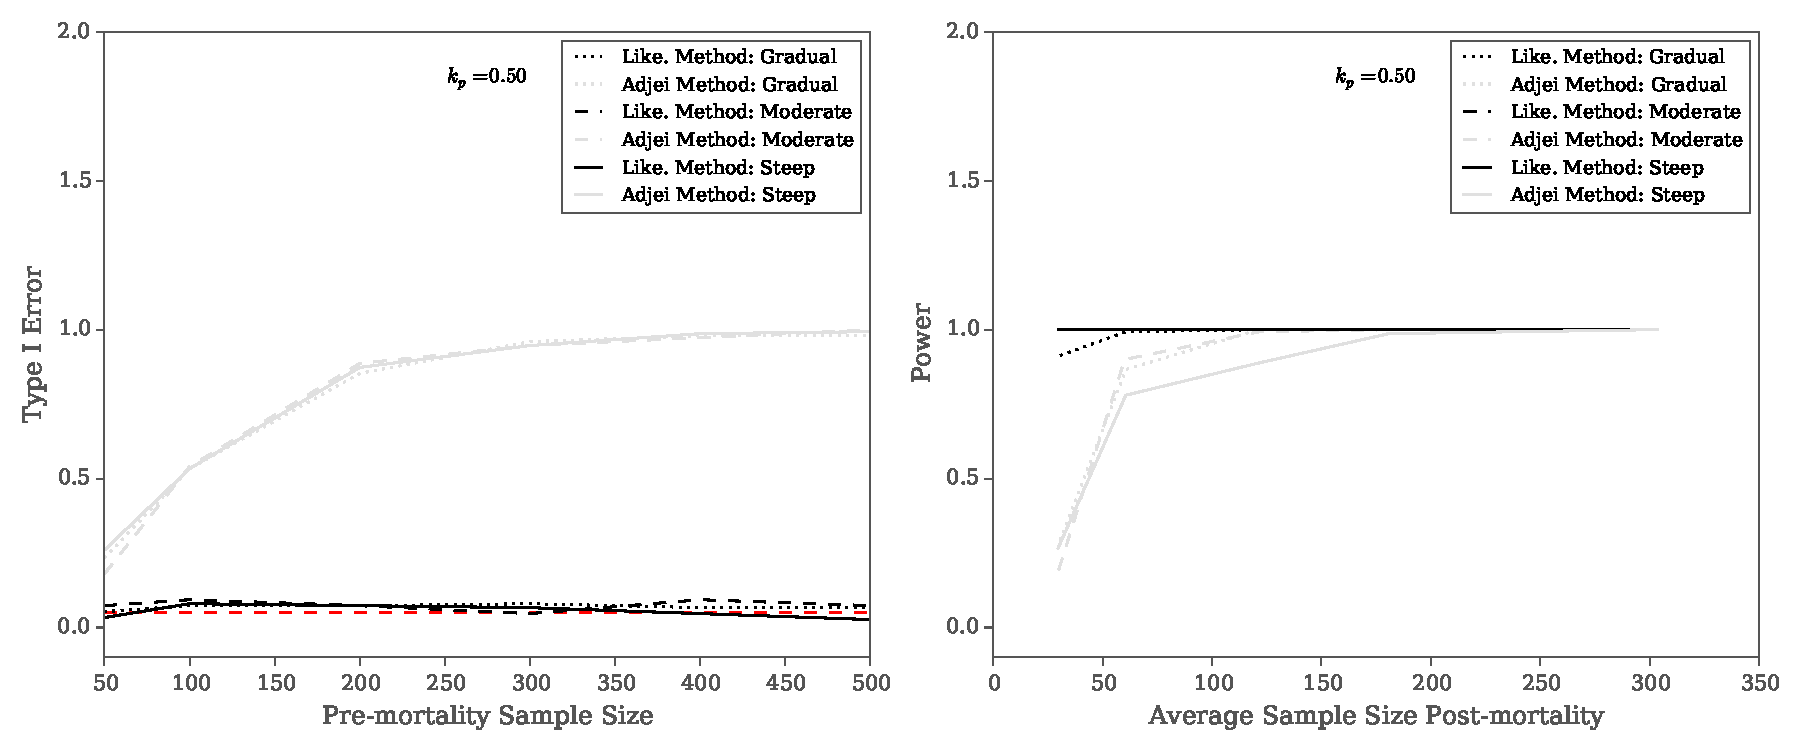
\includegraphics[width=\textwidth]{/Users/mqwilber/Repos/parasite_mortality/results/figure1_partII_for_manuscript50}};

    \node[above=0.1cm] at (pic.north) (concept) {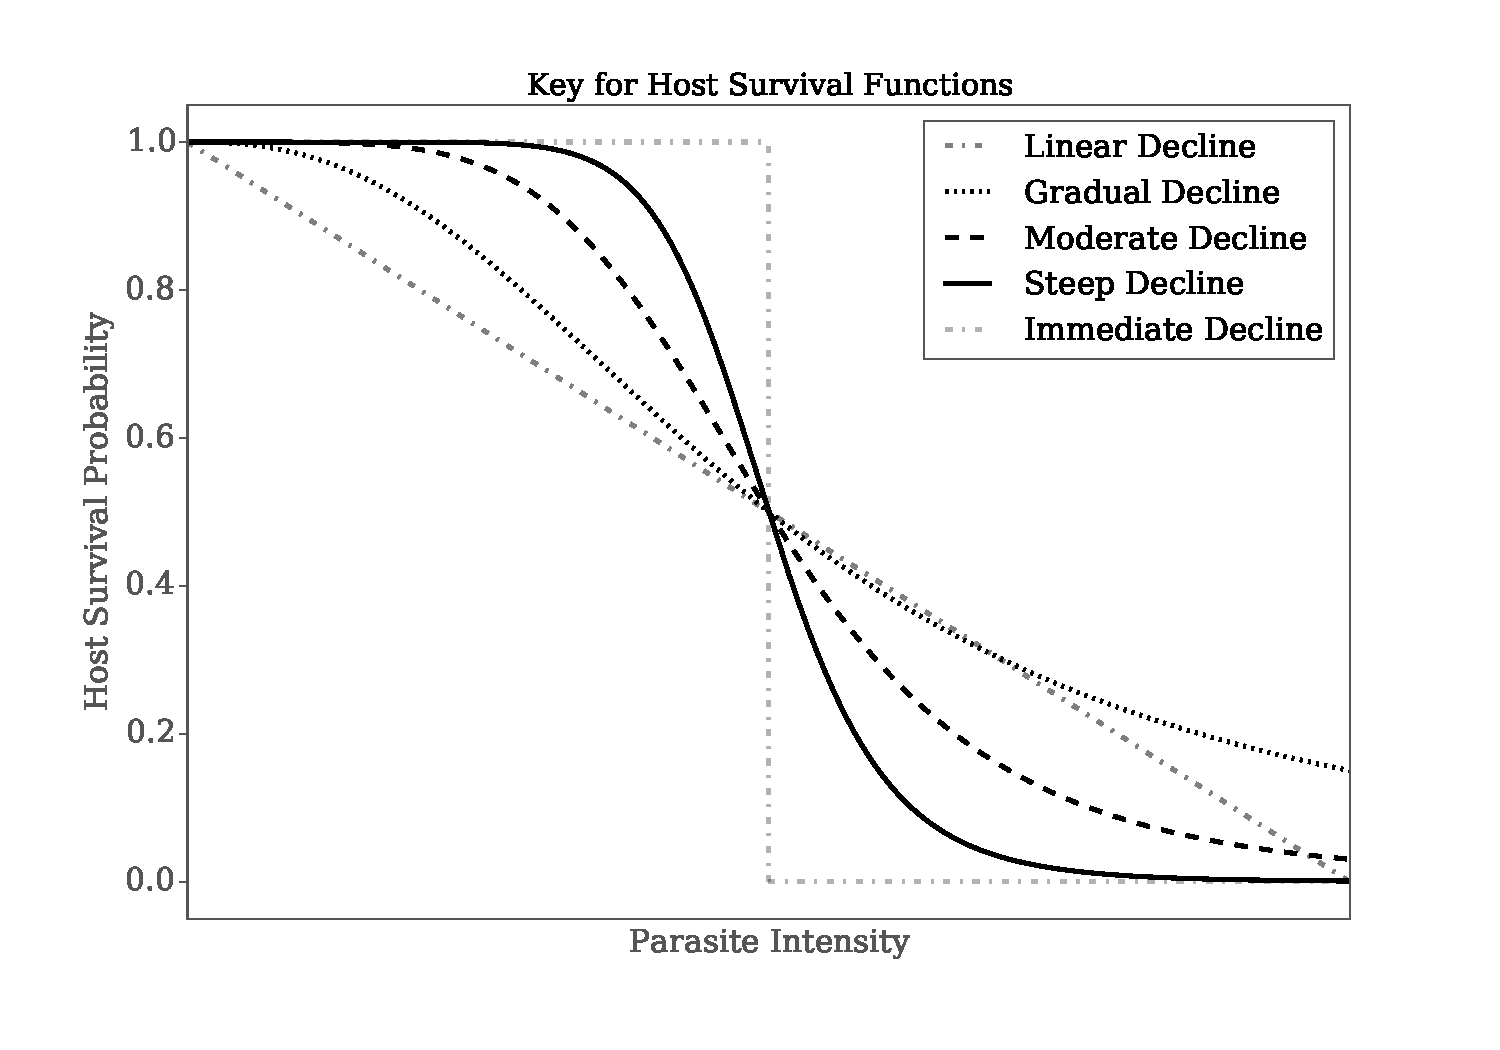
\includegraphics[width=0.6\textwidth]{/Users/mqwilber/Repos/parasite_mortality/results/figure1_partI_for_manuscript}};

    \draw[->] (0, 4.2)--(-1.5, 3.1);
    \draw[->] (0, 4.2)--(1.5, 3.1);

    \node at (-3.2, 4.9) {A.};
    \node at (-6.5, 2.7) {B.};
    \node at (1.4, 2.7) {C.};

\end{tikzpicture}

\caption{A) Five potential shapes for a host-survival functions. In the simulations we used a gradual survival function (dotted line), and moderate survival function (dashed line), and a steep survival function (solid line). The linear and immediate survival functions represent two potential extremes that we do not include in the simulations. For each of these survival functions and the parameter combinations described in the main text, we tested the Type I error and power of the Likelihood Method and Adjei Method. B) Gives the Type I error of each method over a range of pre-mortality sample sizes with a pre-mortality mean parasite intensity ($\mu_p$) of 50 and pre-mortality parasite aggregation ($k_p$) at 0.5. The red line shows the pre-set significance level of 0.05. C) Gives the Power of each method for detecting PIHM over a range of post-mortality sample sizes for $\mu_p = 50$ and $k_p = 0.5$.  In general, the Likelihood Method has higher power and lower Type I error than the Adjei Method.  See the \emph{SI} 3 Fig 1 - 3 for Type I Error and power results for all parameter combinations.}

\label{fig:question1}

\end{figure}

\begin{figure}
    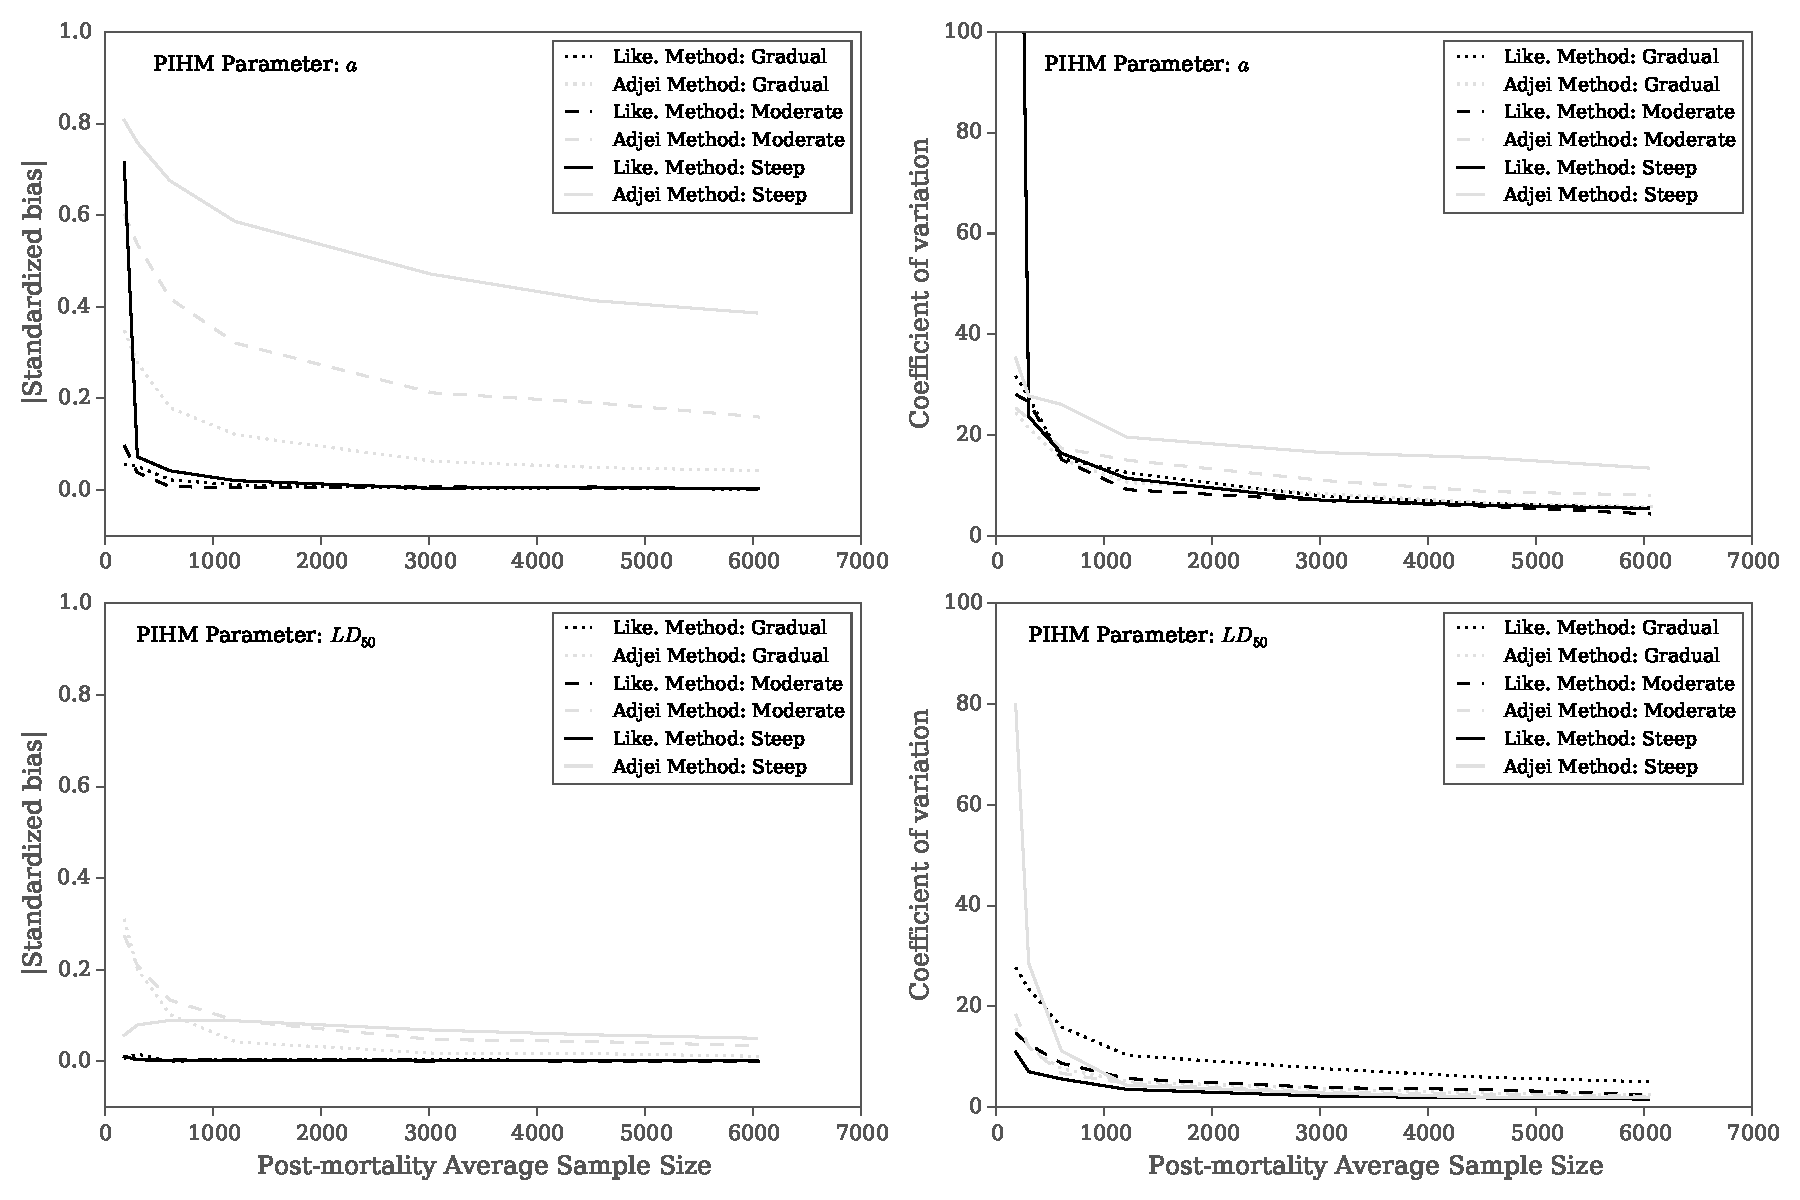
\includegraphics[width=\textwidth]{/Users/mqwilber/Repos/parasite_mortality/results/figure2_for_manuscript.pdf}

    \caption{Bias and precision (coefficient of variation) for the Likelihood Method and Adjei Method estimates of the $a$ parameter and the $LD_{50}$ of the host survival function based on simulated PIHM data over a range of post-mortality sample sizes.  As the coefficient of variation increases, precision decreases. The pre-mortality parameters for this simulation were $\mu_p = 50$ and $k_p = 0.5$.  The figure shows the simulations for three different host survival functions (gradual, moderate, and steep), each with the same $LD_{50}$.  Bias and precision results of $LD_{50}$ and $a$ for all other parameter combinations can be found in \emph{SI} 3 Fig 4 - 9.}

    \label{fig:question2}

\end{figure}

\begin{figure}
    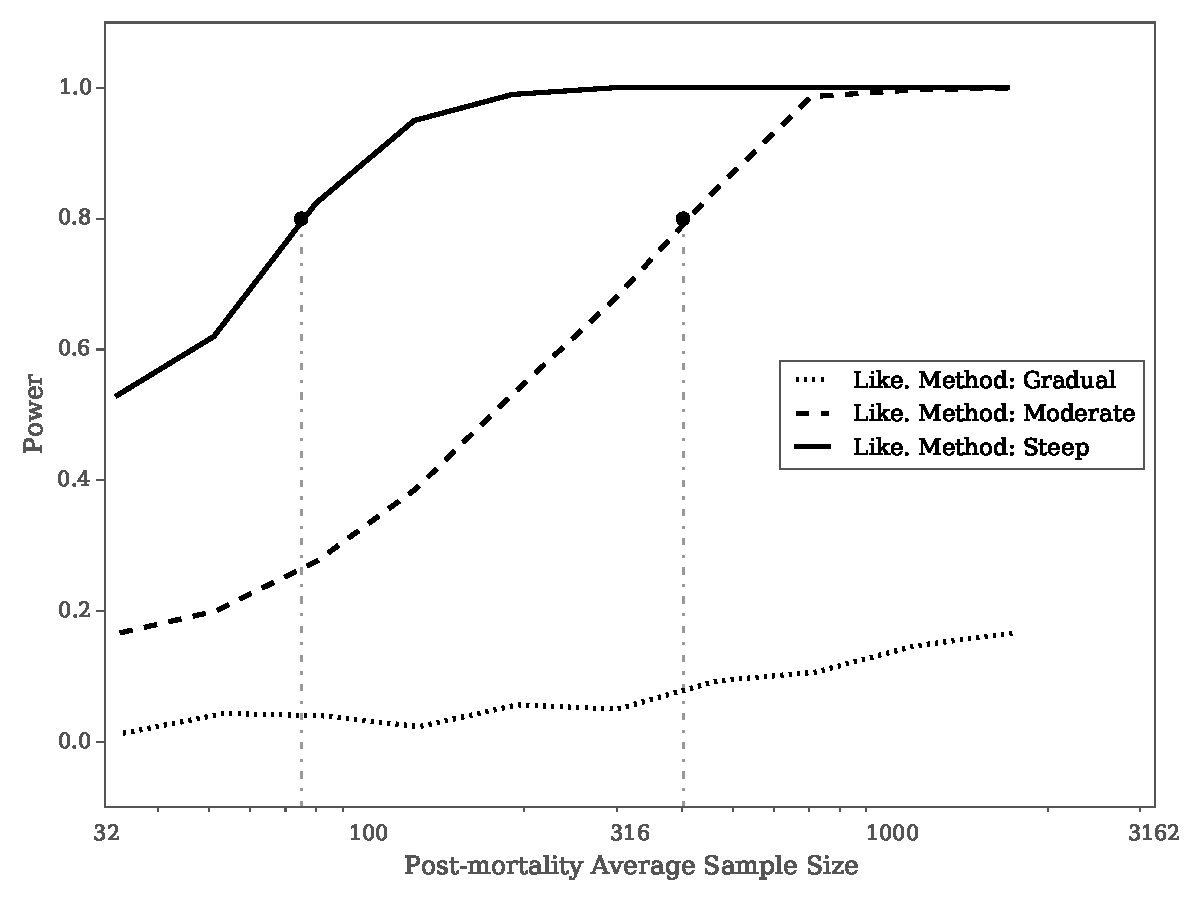
\includegraphics[width=\textwidth]{/Users/mqwilber/Repos/parasite_mortality/results/figure3_for_manuscript.pdf}

    \caption{The power of the Likelihood Method to detect PIHM for gradual, moderate, and steep survival functions when all four parameters $\mu_p$, $k_p$, $a$, and $b$ were jointly estimated. The curves were generated from 500 simulations for 10 pre-mortality population sizes, $N_p$.}

    \label{fig:real_power}

\end{figure}


\end{document}

